\documentclass[
11pt, % The default document font size, options: 10pt, 11pt, 12pt
%codirector, % Uncomment to add a codirector to the title page
]{charter} 


% El títulos de la memoria, se usa en la carátula y se puede usar el cualquier lugar del documento con el comando \ttitle
\titulo{Detección automatizada de patologías pulmonares en rayos X} 

% Nombre del posgrado, se usa en la carátula y se puede usar el cualquier lugar del documento con el comando \degreename
\posgrado{Carrera de Especialización en Sistemas Embebidos} 
%\posgrado{Carrera de Especialización en Internet de las Cosas} 
%\posgrado{Carrera de Especialización en Inteligencia Artificial}
%\posgrado{Maestría en Sistemas Embebidos} 
%\posgrado{Maestría en Internet de las cosas}

% Tu nombre, se puede usar el cualquier lugar del documento con el comando \authorname
% IMPORTANTE: no omitir titulaciones ni tildación en los nombres, también se recomienda escribir los nombres completos (tal cual los tienen en su documento)
\autor{Ing. Rodrigo Nicolás Lauro}

% El nombre del director y co-director, se puede usar el cualquier lugar del documento con el comando \supname y \cosupname y \pertesupname y \pertecosupname
\director{Dr. Facundo Adrián Lucianna}
\pertenenciaDirector{FIUBA} 
\codirector{} % para que aparezca en la portada se debe descomentar la opción codirector en los parámetros de documentclass
\pertenenciaCoDirector{FIUBA}

% Nombre del cliente, quien va a aprobar los resultados del proyecto, se puede usar con el comando \clientename y \empclientename
\cliente{Hospital de Clinicas}
\empresaCliente{Dr. Martin Drago}
 
\fechaINICIO{26 de agosto de 2025}		%Fecha de inicio de la cursada de GdP \fechaInicioName
\fechaFINALPlan{14 de octubre de 2025} 	%Fecha de final de cursada de GdP
\fechaFINALTrabajo{15 de junio de 2026}	%Fecha de defensa pública del trabajo final


\begin{document}

\maketitle
\thispagestyle{empty}
\pagebreak


\thispagestyle{empty}
{\setlength{\parskip}{0pt}
\tableofcontents{}
}
\pagebreak


\section*{Registros de cambios}
\label{sec:registro}


\begin{table}[ht]
\centering
\caption{Registros de cambios}
\label{tab:registro}
\begin{tabularx}{\linewidth}{|c|X|c|}
\hline
\rowcolor[HTML]{C0C0C0} 
Revisión & Detalles de los cambios realizados & Fecha \\ \hline
0 & Creación del documento & 26 de agosto de 2025 \\ \hline
1 & Se completa hasta el punto 5 inclusive & 8 de septiembre de 2025 \\ \hline
2 & Se completa hasta el punto 9 inclusive & 15 de septiembre de 2025 \\ \hline
3 & Se completa hasta el punto 12 inclusive & 22 de septiembre de 2025 \\ \hline
%   Se puede agregar algo más \newline
%   En distintas líneas \newline
%   Así & {día} de {mes} de 202X \\ \hline
%3 & Se completa hasta el punto 12 inclusive & {día} de {mes} de 202X \\ \hline
%4 & Se completa el plan & {día} de {mes} de 202X \\ \hline
\end{tabularx}
\end{table}
\pagebreak

\pagebreak



\section*{Acta de constitución del proyecto}
\label{sec:acta}

\begin{flushright}
Buenos Aires, \fechaInicioName
\end{flushright}

\vspace{2cm}

Por medio de la presente se acuerda con el \authorname\hspace{1px} que su Trabajo Final de la \degreename\hspace{1px} se titulará ``\ttitle'' y consistirá en la implementación de un sistema de soporte a la decisión clínica basado en técnicas de aprendizaje automático. El trabajo tendrá un presupuesto preliminar estimado de 600 horas y un costo estimado de U\$S 45.000,00 , con fecha de inicio el \fechaInicioName\hspace{1px} y fecha de presentación pública el \fechaFinalName.

Se adjunta a esta acta la planificación inicial.

\vfill

% Esta parte se construye sola con la información que hayan cargado en el preámbulo del documento y no debe modificarla
\begin{table}[ht]
\centering
\begin{tabular}{ccc}
\begin{tabular}[c]{@{}c@{}}Dr. Ing. Ariel Lutenberg \\ Director posgrado FIUBA\end{tabular} & \hspace{2cm} & \begin{tabular}[c]{@{}c@{}}\clientename \\ \empclientename \end{tabular} \vspace{2.5cm} \\ 
\multicolumn{3}{c}{\begin{tabular}[c]{@{}c@{}} \supname \\ Director del Trabajo Final\end{tabular}} \vspace{2.5cm} \\
\end{tabular}
\end{table}




\section{1. Descripción técnica-conceptual del proyecto a realizar}
\label{sec:descripcion}


Este proyecto tiene por objetivo ser una herramienta para la detección de patologías pulmonares, basado en rayos X. El mismo se desarrolla en conjunto con el Hospital de Clínicas, responde a una propuesta personal donde se buscó como objetivo principal generar un impacto en la sociedad. En adelante, esta solución se denominará SSDC-RxT (Sistema de Soporte a la Decisión Clínica para Radiografías de Tórax). 

El hospital de clínicas realiza placas de rayos X de torax en todos los pacientes que ingresan, es un procedimiento de rutina. La intención de este proyecto es brindar una herramienta que permita detectar patologías pulmonares (como neumonía, tuberculosis, derrame pleural, cardiomegalia y lesiones pulmonares o mediastinales)  de manera prematura, ya que muchas de esas radiografías no terminan pasando por un experto que pudiera analizarlas. 

De esta manera se estaría generando un fuerte impacto en sectores de la sociedad que no cuentan con recursos para atenderse de manera adecuada. Por otro lado , se le estaría brindando una herramienta al hospital público que sirviera como complemento a sus profesionales.

Este desarrollo se integra como una instancia automática dentro del proceso de admisión. No suma carga operativa: en segundos ofrece un apoyo al médico de guardia y admisión con indicios tempranos y priorización de radiografías potencialmente anómalas, para facilitar decisiones más rápidas. La innovación radica en incorporar soporte diagnóstico temprano directamente en el flujo de trabajo del hospital, como complemento no reemplazo del criterio del especialista.


En la figura 1 se presenta el diagrama en bloques de la solución propuesta. Se observa el flujo completo desde la admisión del paciente y la adquisición de la radiografía, pasando por el preprocesamiento y la clasificación automática mediante IA, hasta la priorización y generación de un reporte breve/alerta para el médico de guardia o especialista.
 
\vspace{25px}
\begin{figure}[htpb]
\centering 
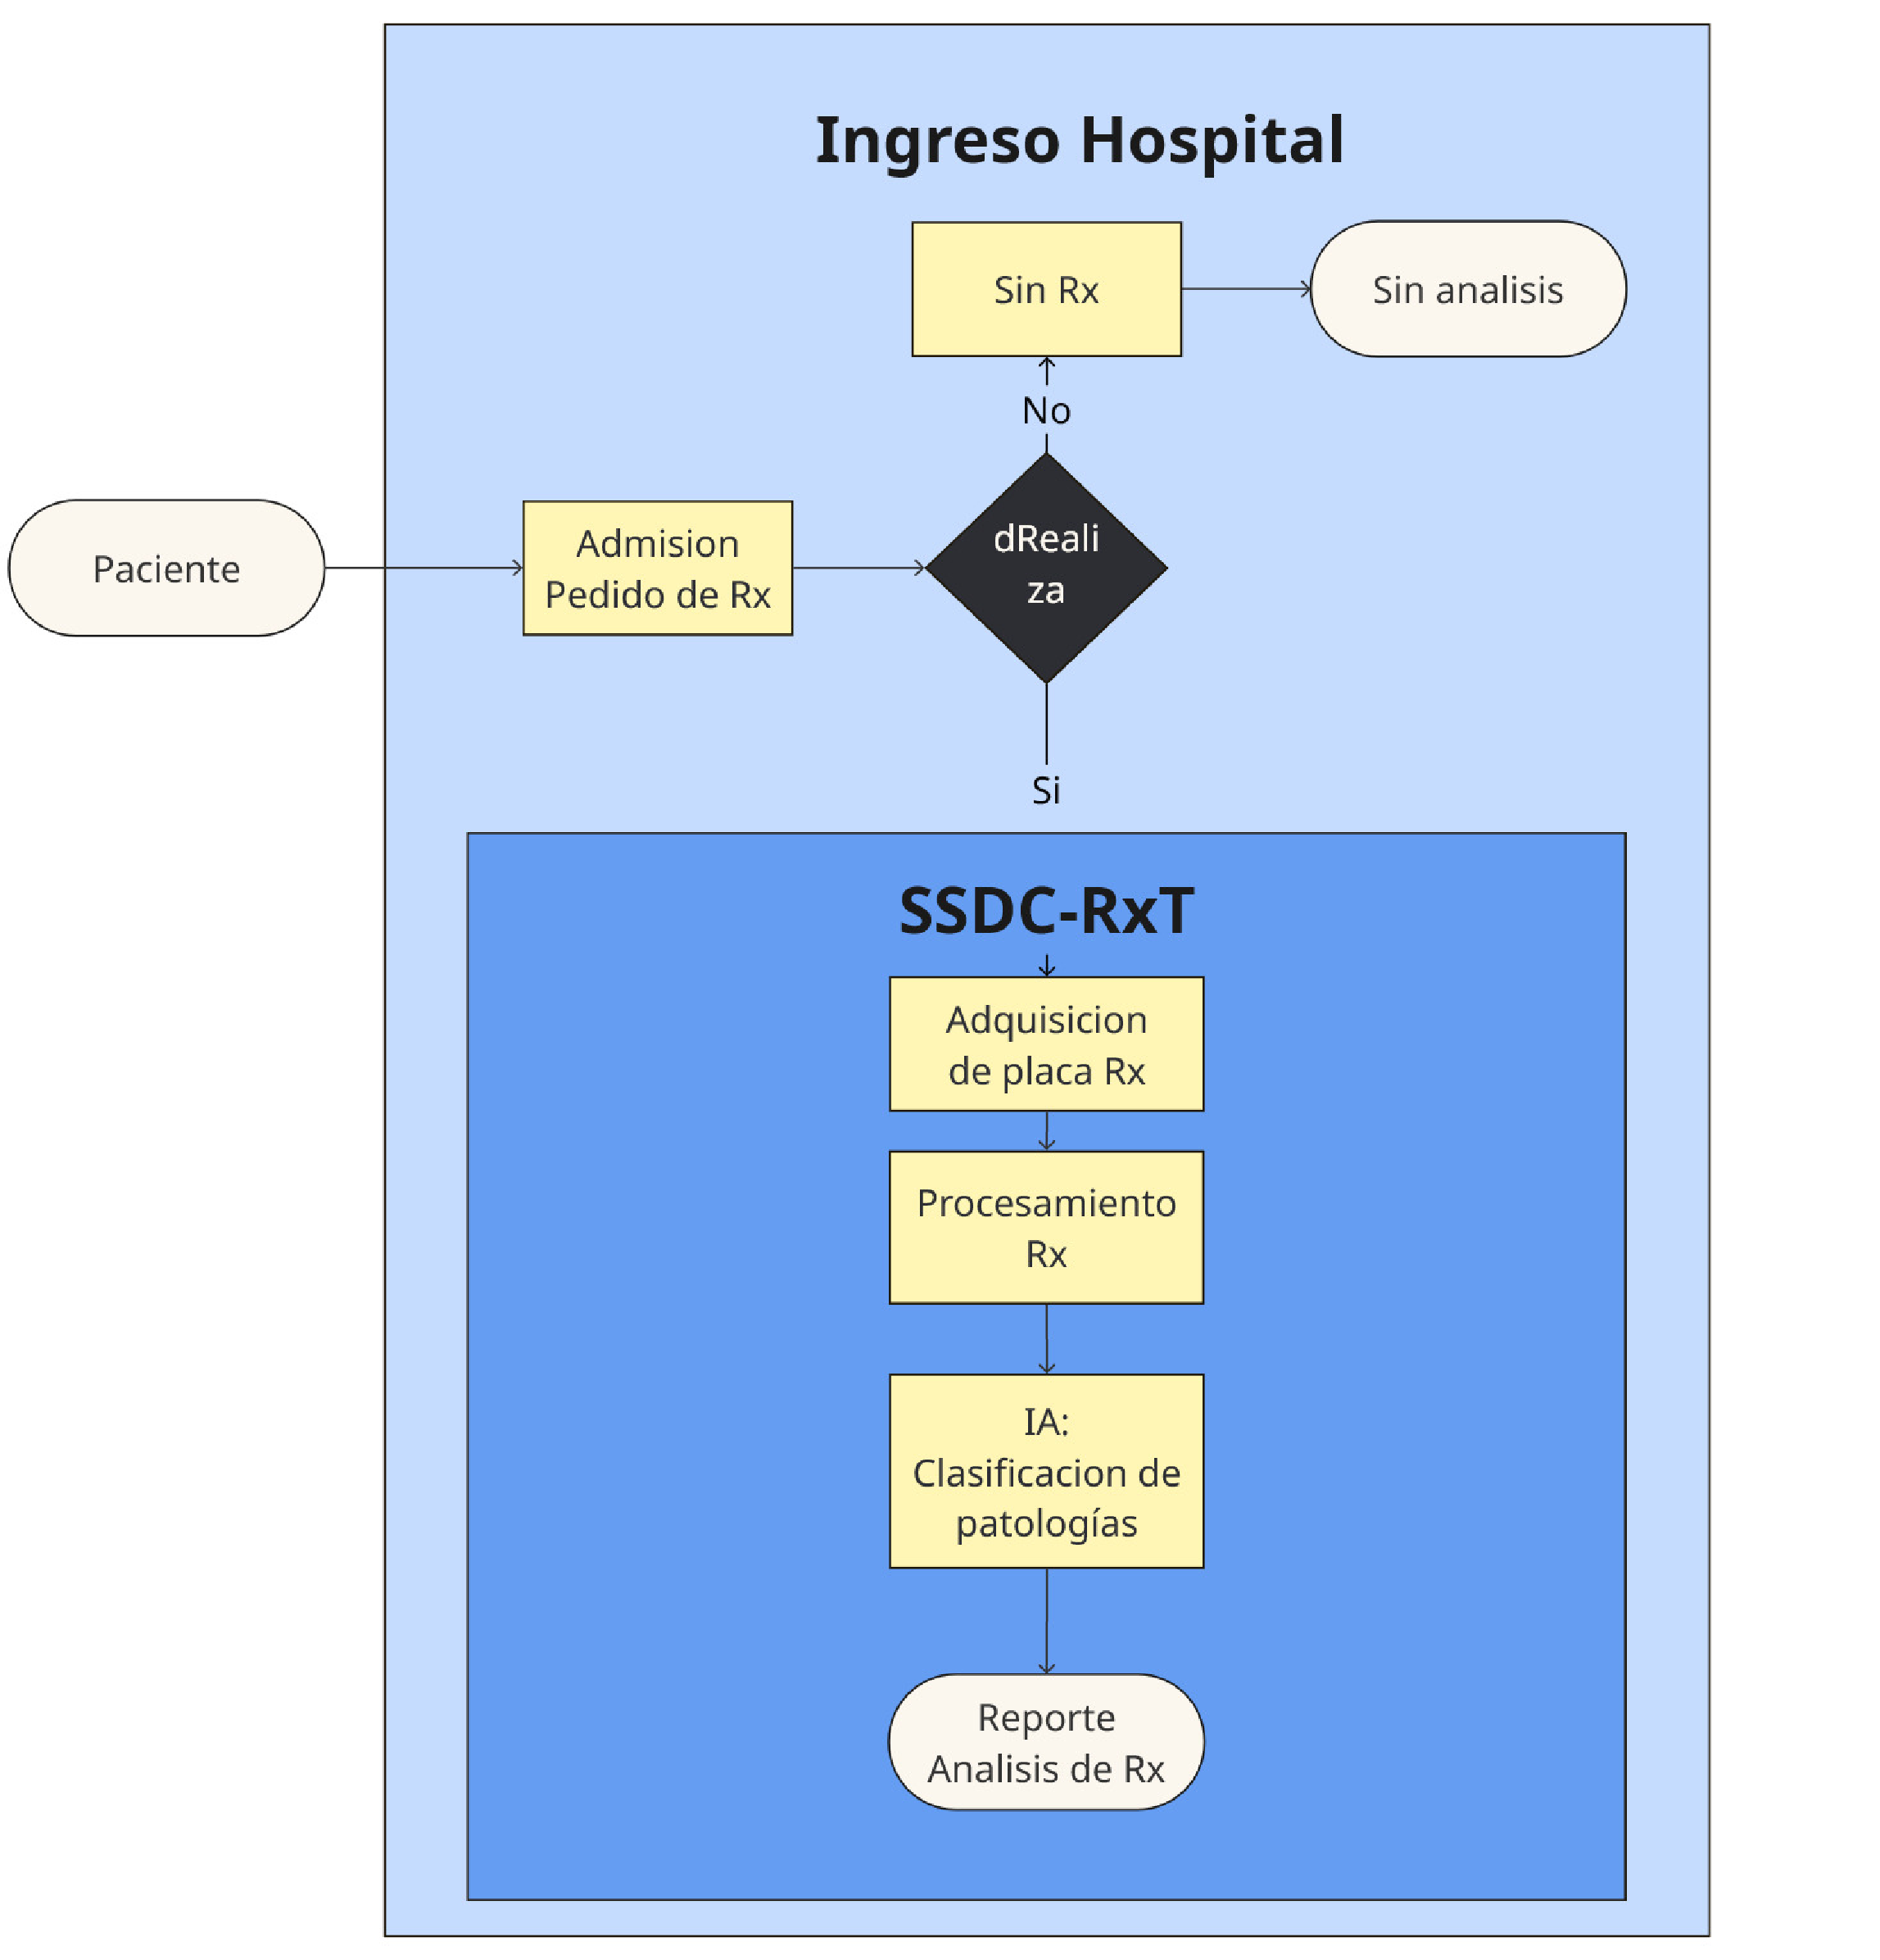
\includegraphics[width=1.1\textwidth]{./Figuras/diagBloques.pdf}
\caption{Diagrama en bloques del SSDC-RxT (sistema propuesto).}
\label{fig:diagBloques}
\end{figure}

\vspace{25px}
\pagebreak




\section{2. Identificación y análisis de los interesados}
\label{sec:interesados}


\begin{table}[ht]
%\caption{Identificación de los interesados}
%\label{tab:interesados}
\begin{tabularx}{\linewidth}{@{}|l|X|X|l|@{}}
\hline
\rowcolor[HTML]{C0C0C0} 
Rol           & Nombre y Apellido & Organización 	& Puesto 	\\ \hline
Cliente       &\clientename      &\empclientename	&       	\\ \hline
Responsable   &\authorname       & FIUBA        	& Ing. Lauro 	\\ \hline
Orientador    &\supname	      & \pertesupname 	& Director del Trabajo Final \\ \hline
Usuario final & Prof. médicos     &\empclientename	&        	\\ \hline
\end{tabularx}
\end{table}


\begin{itemize}
	\item Cliente: el Dr. Martin Drago es experto en la temática y va a ayudar con la creación de un equipo de etiquetado de las patologías.
\end{itemize}



\section{3. Propósito del proyecto}
\label{sec:proposito}

 
Impactar positivamente en la atención, en especial de pacientes de sectores más vulnerables, ofreciendo soporte de  diagnóstico temprano en radiografías de tórax. La solución prioriza automáticamente estudios con hallazgos sospechosos y entrega reportes breves a los médicos, acelerando decisiones, mejorando la detección precoz y optimizando recursos sin sumar carga operativa.
 

\section{4. Alcance del proyecto}
\label{sec:alcance}

El proyecto incluye:
\begin{itemize}
  \item \textbf{Plataforma de etiquetado (portal de especialistas).}
    \begin{itemize}
      \item Gestión de usuarios (médicos/radiólogos) y trazabilidad.
      \item Carga/visualización de Rx (DICOM/JPG) con desidentificación.
      \item Etiquetado multicategoría (neumonía, TB, derrame, cardiomegalia, otras lesiones).
      \item Exportación de etiquetas para entrenamiento (CSV/JSON).
    \end{itemize}
  \item \textbf{\textit{SSDC-RxT}: desarrollo de IA y \textit{pipeline}.}
    \begin{itemize}
      \item Preprocesamiento (control de calidad, normalización, redimensión).
      \item Entrenamiento y validación de modelos de clasificación multiclase.
      \item \textit{Scoring} y priorización de estudios con hallazgos sospechosos.
      \item Métricas de evaluación (AUC, sensibilidad/especificidad por clase, validación cruzada).
      \item Exposición de inferencia vía API REST.
    \end{itemize}
  \item \textbf{Portal clínico (usuarios profesionales).}
    \begin{itemize}
      \item Ingreso/búsqueda de estudios y ejecución de inferencia.
      \item Visualización de resultado, nivel de confianza y prioridad (reporte/alerta).
      \item Control de acceso, registro de actividad y descarga del reporte.
    \end{itemize}
  \item \textbf{Infraestructura y despliegue.}
    \begin{itemize}
      \item Servidor/VM (on-prem o cloud), contenedores (Docker).
      \item \textit{Logging}, monitoreo básico y \textit{backups}.
      \item Versionado de \textit{datasets}/modelos y procedimiento de actualización de modelo.
    \end{itemize}
  \item \textbf{Documentación y pruebas.}
    \begin{itemize}
      \item Manual técnico y de usuario.
      \item Plan y resultados de pruebas funcionales y de desempeño.
    \end{itemize}
\end{itemize}

El presente proyecto no incluye:
\begin{itemize}
  \item Diagnóstico médico final ni reemplazo del especialista.
  \item Certificación regulatoria (ANMAT/CE/FDA) ni trámites legales asociados.
  \item Integración productiva completa con HIS/RIS/PACS; se limita a un piloto/PoC con importación/exportación básica.
  \item Adquisición de equipamiento de rayos X ni modificaciones de hardware existente.
  \item Operación 24x7, mesa de ayuda o mantenimiento continuo más allá de la fase piloto.
  \item Aplicaciones móviles nativas; el alcance se limita a interfaz web.
  \item Entrenamiento desde cero de modelos fundacionales ni cómputo distribuido; se usarán modelos preentrenados con \textit{fine-tuning}.
  \item Gestión avanzada de consentimiento/ética más allá de desidentificación y resguardos internos establecidos.
\end{itemize}



\section{5. Supuestos del proyecto}
\label{sec:supuestos}
 
El proyecto se apoya en los siguientes supuestos:
\begin{itemize}
  \item \textbf{Datos y acceso.}
    \begin{itemize}
      \item Disponibilidad de acceso a placas de radiografías de tórax (históricas y nuevas) en formato DICOM/JPG.
      \item Volumen y diversidad suficientes para entrenar, validar y probar el modelo (clases representadas, distribución razonable).
      \item Posibilidad de exportar desde PACS/RIS y de desidentificar los estudios antes de su uso.
      \item Disponibilidad de metadatos clínicos básicos (p.\,ej., proyección PA/AP, sexo, edad aproximada) cuando sea pertinente y permitido.
    \end{itemize}

    \pagebreak
    
  \item \textbf{Etiquetado por expertos.}
    \begin{itemize}
      \item Participación de médicos/radiólogos del Hospital de Clínicas como \emph{gold standard} para el etiquetado.
      \item Tiempo asignado para etiquetar conforme a un protocolo consensuado.
      \item Mecanismo de resolución de discrepancias (doble lectura y, si aplica, tercer lector); concordancia interobservador mínima aceptable.
    \end{itemize}  
      \item Aprobación institucional/comité de ética para uso de datos desidentificados con fines de investigación/piloto.
      \item Cumplimiento de normativa de protección de datos aplicable y políticas internas (acceso por roles, auditoría).
    \end{itemize}
  \item \textbf{Operación y adopción.}
    \begin{itemize}
      \item Disponibilidad de los profesionales para una breve capacitación y uso del portal clínico.
      \item Aceptación del flujo de trabajo propuesto (alertas/priorización) sin cambios mayores en protocolos asistenciales.
      \item Respaldo de jefaturas/gestión para ejecutar el piloto en el ámbito acordado.
    \end{itemize}
  
\end{itemize}

\section{6. Product Backlog}
\label{sec:backlog}

\subsection*{Épica 1 – Gestión y etiquetado de radiografías}

\textbf{HU1}  
Como especialista, quiero cargar radiografías de tórax en el sistema para poder etiquetarlas con patologías relevantes.  
\\Dificultad: 3, Complejidad: 3, Incertidumbre: 2 → Suma: 8 → \textbf{Story Points: 8}  
Prioridad: Alta  

\textbf{HU2}  
Como especialista, quiero registrar múltiples etiquetas por cada radiografía para reflejar la presencia de más de una patología.  
\\Dificultad: 5, Complejidad: 3, Incertidumbre: 5 → Suma: 10 → \textbf{Story Points: 13}  
Prioridad: Alta  

\subsection*{Épica 2 – Entrenamiento y validación del modelo IA}

\textbf{HU3}  
Como desarrollador, quiero entrenar un modelo de clasificación multiclase con las radiografías etiquetadas para detectar patologías pulmonares de forma automática.  
\\Dificultad: 5, Complejidad: 5, Incertidumbre: 3 → Suma: 13 → \textbf{Story Points: 13}  
Prioridad: Alta  

\textbf{HU4}  
Como desarrollador, quiero validar el modelo con un conjunto de datos separado para asegurar que los resultados sean confiables.  
\\Dificultad: 3, Complejidad: 3, Incertidumbre: 2 → Suma: 8 → \textbf{Story Points: 8}  
Prioridad: Alta  

\subsection*{Épica 3 – Portal clínico de soporte al diagnóstico}

\textbf{HU5}  
Como médico de guardia, quiero subir una radiografía de un paciente para recibir un resultado automático que me ayude en la admisión.  
\\Dificultad: 5, Complejidad: 3, Incertidumbre: 3 → Suma: 11 → \textbf{Story Points: 13}  
Prioridad: Alta  

\textbf{HU6}  
Como médico de guardia, quiero que el sistema me muestre un nivel de confianza y prioridad de cada caso para tomar decisiones más rápidas.  
\\Dificultad: 5, Complejidad: 5, Incertidumbre: 3 → Suma: 13 → \textbf{Story Points: 13}  
Prioridad: Alta  

\subsection*{Épica 4 – Infraestructura y seguridad del sistema}

\textbf{HU7}  
Como administrador, quiero que el sistema funcione en un servidor seguro para garantizar el resguardo de datos médicos.  
\\Dificultad: 3, Complejidad: 4, Incertidumbre: 3 → Suma: 10 → \textbf{Story Points: 13}  
Prioridad: Alta  

\textbf{HU8}  
Como administrador, quiero que los accesos estén diferenciados por roles para asegurar que solo los usuarios autorizados utilicen el sistema.  
\\Dificultad: 3, Complejidad: 3, Incertidumbre: 2 → Suma: 8 → \textbf{Story Points: 8}  
Prioridad: Alta  


\section{7. Criterios de aceptación de historias de usuario}
\label{sec:criteriosAceptacion}

\section{Criterios de aceptación}

\subsection*{Épica 1 – Gestión y etiquetado de radiografías}

\textbf{Criterios de aceptación HU1} (Carga de Rx para etiquetar)
\begin{itemize}
  \item Se permite cargar archivos DICOM/JPG válidos y de tamaño controlado.
  \item Al finalizar la carga, el estudio queda disponible en el listado de “Pendientes de etiquetar”.
  \item Se almacenan los archivos de manera desidentificada y con registro de auditoría.
\end{itemize}

\textbf{Criterios de aceptación HU2} (Etiquetado multicategoría)
\begin{itemize}
  \item Es posible asignar múltiples etiquetas por estudio en una sola acción.
  \item Las etiquetas aplicadas se muestran de forma clara en la interfaz y cambian el estado a “Etiquetada”.
  \item Se conserva el historial de etiquetas y, cuando corresponde, se registra la concordancia entre lectores.
\end{itemize}

\subsection*{Épica 2 – Entrenamiento y validación del modelo IA}

\textbf{Criterios de aceptación HU3} (Entrenar modelo multiclase)
\begin{itemize}
  \item Se separan previamente los datos en conjuntos de entrenamiento, validación y prueba.
  \item El modelo se entrena únicamente con el conjunto de entrenamiento (usando validación para ajuste de hiperparámetros).
  \item Se genera un artefacto de modelo versionado y exportable.
  \item Se produce un reporte automático con métricas del entrenamiento (curvas ROC, matriz de confusión en validación).
\end{itemize}

\textbf{Criterios de aceptación HU4} (Validación con conjunto separado)
\begin{itemize}
  \item La evaluación se realiza exclusivamente sobre este conjunto, generando métricas por clase y globales (AUC, sensibilidad, especificidad, F1).
  \item Los resultados alcanzan al menos los umbrales mínimos establecidos en la fase de Evaluación de CRISP-DM (ej.: AUC macro ≥ 0,85; sensibilidad por clase ≥ 0,75).
  \item Se cumplen umbrales mínimos definidos (ej. AUC macro ≥ 0,85).
\end{itemize}



\subsection*{Épica 3 – Portal clínico de soporte al diagnóstico}

\textbf{Criterios de aceptación HU5} (Subir Rx y obtener resultado)
\begin{itemize}
  \item El usuario puede subir una Rx y obtener predicciones en menos de 10 segundos.
  \item La interfaz indica claramente el estado de procesamiento y el resultado final.
  \item Cada ejecución queda registrada con usuario, fecha y resultado.
\end{itemize}

\textbf{Criterios de aceptación HU6} (Confianza y priorización)
\begin{itemize}
  \item El sistema muestra el nivel de confianza de cada predicción.
  \item Los casos se ordenan según prioridad y se resaltan con un código visual.
  \item Se mantienen configurables los umbrales que determinan las prioridades.
\end{itemize}

\subsection*{Épica 4 – Infraestructura y seguridad del sistema}

\textbf{Criterios de aceptación HU7} (Servidor seguro)
\begin{itemize}
  \item El sistema está desplegado en un servidor/VM con acceso restringido y comunicaciones cifradas mediante TLS 1.3.
  \item Existe una página de estado con la versión del modelo y disponibilidad del servicio.
  \item Los datos y modelos se almacenan con cifrado AES-256 en reposo y claves gestionadas de forma segura.
  \item Se ejecutan backups diarios automáticos, validados con checksums (SHA-256) y verificados mediante pruebas de restauración periódicas bajo la regla 3-2-1.
\end{itemize}



\textbf{Criterios de aceptación HU8} (Accesos por roles)
\begin{itemize}
  \item Se definen roles diferenciados (administrador, especialista, médico) con permisos específicos.
  \item La interfaz se adapta a cada rol mostrando solo las opciones disponibles.
  \item El sistema registra los intentos de acceso y bloquea tras varios fallidos.
\end{itemize}


\section{8. Fases de CRISP-DM}

\subsection*{1. Comprensión del negocio}
\begin{itemize}
  \item \textbf{Objetivo:} priorizar tempranamente radiografías de tórax con hallazgos sospechosos para asistir la decisión clínica en admisión/guardia.
  \item \textbf{Valor agregado:} Reducción del tiempo hasta la atención de casos críticos; soporte sistemático y trazable sin aumentar carga operativa.
  \item \textbf{Métricas de éxito (negocio):} 
    \begin{itemize}
      \item TTR (time-to-review) de placas prioritarias: reducción \(\geq\) 30\%.
      \item \% de casos críticos correctamente priorizados: \(\geq\) 85\%.
      \item Adopción por parte de médicos de guardia: \(\geq\) 70\% en piloto.
    \end{itemize}
\end{itemize}

\subsection*{2. Comprensión de los datos}
\begin{itemize}
  \item \textbf{Tipo:} Imágenes Rx de tórax (DICOM/JPG), metadatos (proyección PA/AP, sexo, edad aprox. cuando esté permitido).
  \item \textbf{Origen:} Hospital de Clínicas (PACS/RIS). Etiquetas provistas por especialistas del hospital.
  \item \textbf{Cantidad esperada:} Centenares a miles de estudios para piloto (balance por clase a verificar).
  \item \textbf{Calidad:} Variabilidad de equipos y parámetros; posibles artefactos. Se requiere control de calidad y desidentificación.
\end{itemize}

\subsection*{3. Preparación de los datos}
\begin{itemize}
  \item \textbf{Características clave:} Imagen normalizada (tamaño fijo, 1 o 3 canales), proyección conocida, etiquetas multicategoría.
  \item \textbf{Transformaciones:} 
    \begin{itemize}
      \item Desidentificación, control de calidad (descartar estudios inválidos).
      \item Normalización de intensidades, \textit{resize}/centrado, data augmentation limitado.
      \item Split estratificado: train/val/test sin fuga de información.
    \end{itemize}
\end{itemize}

\subsection*{4. Modelado}
\begin{itemize}
  \item \textbf{Tipo de problema:} Clasificación multiclase/multietiqueta de patologías en Rx de tórax con \textbf{scoring} de prioridad.
  \item \textbf{Algoritmos posibles:} 
    \begin{itemize}
      \item CNN con \textit{transfer learning} (p.ej., EfficientNet/ResNet) + \textit{fine-tuning}.
      \item Clasificadores calibrados para probabilidades (p.ej., \textit{temperature scaling} si aplica).
    \end{itemize}
  \item \textbf{Selección/ajuste:} Búsqueda de hiperparámetros, \textit{early stopping}, regularización; versión de modelo registrada.
\end{itemize}

\subsection*{5. Evaluación del modelo}
\begin{itemize}
  \item \textbf{Métricas de rendimiento (técnicas):} AUC por clase y macro, sensibilidad/especificidad por clase, F1 macro, matriz de confusión.
  \item \textbf{Criterios mínimos (piloto):} AUC macro \(\geq\) 0,85; sensibilidad por clase \(\geq\) 0,75 (valores a consensuar con clínica).
  \item \textbf{Verificación clínica:} Revisión de falsos positivos/negativos y acuerdo interobservador.
\end{itemize}

\subsection*{6. Despliegue del modelo (opcional en piloto)}
\begin{itemize}
  \item \textbf{Tipo de despliegue:} Servicio de inferencia vía API REST (\textit{container} Docker) en servidor/VM del hospital (on-prem o cloud privada).
  \item \textbf{Herramientas:} Contenedores, \textit{artifact store} para versión de modelo, \textit{logging}/auditoría y \textit{health-checks}.
  \item \textbf{Operación del piloto:} Tiempos de respuesta \(\leq\) 10 s, \textit{roll-back} de modelo, umbrales de prioridad configurables.
\end{itemize}


\section{9. Desglose del trabajo en tareas}

A continuación se presenta el desglose de tareas técnicas a partir de las Historias de Usuario (HU) definidas en el Product Backlog (Sección 6). 
Cada tarea tiene una estimación horaria y prioridad relativa.

\begin{center}
\begin{tabular}{|l|p{8.5cm}|c|c|}
\hline
\textbf{Historia de usuario} & \textbf{Tarea técnica} & \textbf{Estimación} & \textbf{Prioridad} \\
\hline
HU1 & Implementar módulo de carga de archivos DICOM/JPG con validación de formato & 7 h & Alta \\
\hline
HU1 & Guardar archivos en repositorio desidentificado con registro de auditoría & 8 h & Alta \\
\hline
HU1 & Vista de “Pendientes de etiquetar” con paginado y búsqueda & 6 h & Media \\
\hline
HU2 & Diseñar interfaz para asignar múltiples etiquetas por estudio & 6 h & Alta \\
\hline
HU2 & Persistir etiquetas en base de datos con control de versiones & 7 h & Alta \\
\hline
HU2 & Exportar etiquetas a CSV/JSON para entrenamiento del modelo & 5 h & Media \\
\hline
HU3 & Configurar pipeline de preprocesamiento (resize, normalización, augmentation) & 8 h & Alta \\
\hline
HU3 & Implementar script de entrenamiento inicial con modelo base (ResNet/EfficientNet) & 8 h & Alta \\
\hline
HU3 & Registrar hiperparámetros y métricas de entrenamiento (logging) & 6 h & Media \\
\hline
HU4 & Dividir dataset en train/val/test de forma estratificada & 5 h & Alta \\
\hline
HU4 & Generar reporte automático con métricas (ROC, matriz de confusión, F1) & 7 h & Alta \\
\hline
HU5 & Programar endpoint de inferencia para subir Rx y ejecutar modelo & 7 h & Alta \\
\hline
HU5 & Desarrollar interfaz web para mostrar resultados al usuario & 6 h & Alta \\
\hline
HU5 & Guardar resultados de inferencia en base de datos para auditoría & 6 h & Media \\
\hline
HU6 & Implementar cálculo de nivel de confianza de predicción & 6 h & Alta \\
\hline
HU6 & Configurar priorización automática con umbrales por clase & 7 h & Alta \\
\hline
HU6 & Mostrar ordenamiento visual de estudios según criticidad & 5 h & Media \\
\hline
HU7 & Configurar despliegue en servidor/VM con Docker & 8 h & Alta \\
\hline
HU7 & Implementar página de estado y health-check del servicio & 6 h & Media \\
\hline
HU7 & Automatizar backup inicial de modelos y datos & 6 h & Media \\
\hline
HU8 & Definir roles (admin, especialista, médico) y permisos asociados & 7 h & Alta \\
\hline
HU8 & Implementar autenticación con sesiones y expiración por inactividad & 7 h & Alta \\
\hline
\end{tabular}
\end{center}



 

\section{10. Planificación de Sprints}


\begin{table}[htpb]
\centering
\caption{Planificación de Sprints (600 h estimadas)}
\begin{tabularx}{\linewidth}{@{}|l|l|X|c|l|c|@{}}
\hline
\rowcolor[HTML]{C0C0C0}
Sprint & HU o fase & Tarea & Horas & Responsable & \% Completado \\ \hline
Sprint 0 & Planificación & Definir alcance y cronograma & 10 h & Ing. Lauro & 100\% \\ \hline
Sprint 0 & Planificación & Reunión con tutor/cliente & 5 h & Ing. Lauro & 50\% \\ \hline
Sprint 0 & Planificación & Ajuste de entregables y setup inicial & 10 h & Ing. Lauro & 25\% \\ \hline
Sprint 1 & HU1 & Implementar módulo de carga DICOM/JPG & 10 h & Ing. Lauro & 0\% \\ \hline
Sprint 1 & HU1 & Guardar archivos desidentificados con auditoría & 10 h & Ing. Lauro & 0\% \\ \hline
Sprint 1 & HU1 & Vista de “Pendientes de etiquetar” & 8 h & Ing. Lauro & 0\% \\ \hline
Sprint 2 & HU2 & Diseñar interfaz para múltiples etiquetas & 12 h & Ing. Lauro & 0\% \\ \hline
Sprint 2 & HU2 & Persistir etiquetas con control de versiones & 10 h & Ing. Lauro & 0\% \\ \hline
Sprint 2 & HU2 & Exportar etiquetas a CSV/JSON & 8 h & Ing. Lauro & 0\% \\ \hline
Sprint 3 & HU3 & Pipeline de preprocesamiento (resize, normalización, augmentation) & 15 h & Ing. Lauro & 0\% \\ \hline
Sprint 3 & HU3 & Script de entrenamiento inicial (ResNet/EfficientNet) & 20 h & Ing. Lauro & 0\% \\ \hline
Sprint 3 & HU3 & Registrar hiperparámetros y métricas de entrenamiento & 10 h & Ing. Lauro & 0\% \\ \hline
Sprint 4 & HU4 & Split estratificado train/val/test & 8 h & Ing. Lauro & 0\% \\ \hline
Sprint 4 & HU4 & Generar reporte automático de métricas (ROC, F1, confusión) & 15 h & Ing. Lauro & 0\% \\ \hline
Sprint 4 & HU4 & Tablero descargable con métricas por clase y macro & 12 h & Ing. Lauro & 0\% \\ \hline
\end{tabularx}
\end{table}




\begin{table}[htpb]
\centering
\begin{tabularx}{\linewidth}{@{}|l|l|X|c|l|c|@{}}
\hline
\rowcolor[HTML]{C0C0C0}
Sprint & HU o fase & Tarea & Horas & Responsable & \% Completado \\ \hline
Sprint 5 & HU5 & Endpoint de inferencia para subir Rx y ejecutar modelo & 15 h & Ing. Lauro & 0\% \\ \hline
Sprint 5 & HU5 & Interfaz web para mostrar resultados al usuario & 12 h & Ing. Lauro & 0\% \\ \hline
Sprint 5 & HU5 & Guardar resultados de inferencia en base de datos & 10 h & Ing. Lauro & 0\% \\ \hline
Sprint 6 & HU6 & Cálculo de nivel de confianza de predicción & 12 h & Ing. Lauro & 0\% \\ \hline
Sprint 6 & HU6 & Priorización automática con umbrales por clase & 15 h & Ing. Lauro & 0\% \\ \hline
Sprint 6 & HU6 & Mostrar ordenamiento visual de estudios según criticidad & 10 h & Ing. Lauro & 0\% \\ \hline
Sprint 7 & HU7 & Configurar despliegue en servidor/VM con Docker & 15 h & Ing. Lauro & 0\% \\ \hline
Sprint 7 & HU7 & Página de estado y health-check del servicio & 10 h & Ing. Lauro & 0\% \\ \hline
Sprint 7 & HU7 & Automatizar backups diarios y verificación de restore & 12 h & Ing. Lauro & 0\% \\ \hline
Sprint 8 & HU8 & Definir roles (admin, especialista, médico) y permisos & 12 h & Ing. Lauro & 0\% \\ \hline
Sprint 8 & HU8 & Autenticación con sesiones y expiración por inactividad & 12 h & Ing. Lauro & 0\% \\ \hline
Sprint 8 & HU8 & Bloqueo tras intentos fallidos y auditoría de accesos & 10 h & Ing. Lauro & 0\% \\ \hline
Sprint 9 & Pruebas & Pruebas integradas de HU1–HU8 & 20 h & Ing. Lauro & 0\% \\ \hline
Sprint 9 & Pruebas & Corrección de errores y ajustes funcionales & 20 h & Ing. Lauro & 0\% \\ \hline
Sprint 9 & Documentación & Documentación técnica de módulos implementados & 15 h & Ing. Lauro & 0\% \\ \hline
\end{tabularx}
\end{table}



\begin{table}[htpb]
\centering
\begin{tabularx}{\linewidth}{@{}|l|l|X|c|l|c|@{}}
\hline
\rowcolor[HTML]{C0C0C0}
Sprint & HU o fase & Tarea & Horas & Responsable & \% Completado \\ \hline
Sprint 10 & Escritura & Redacción memoria: capítulos introductorios y estado del arte & 30 h & Ing. Lauro & 0\% \\ \hline
Sprint 10 & Escritura & Redacción memoria: desarrollo, resultados y conclusiones & 40 h & Ing. Lauro & 0\% \\ \hline
Sprint 10 & Defensa & Preparación de la exposición y práctica de defensa & 20 h & Ing. Lauro & 0\% \\ \hline
\end{tabularx}
\end{table}





\section{11. Diagrama de Gantt (sprints)}

\begin{figure}[ht]
    \centering
    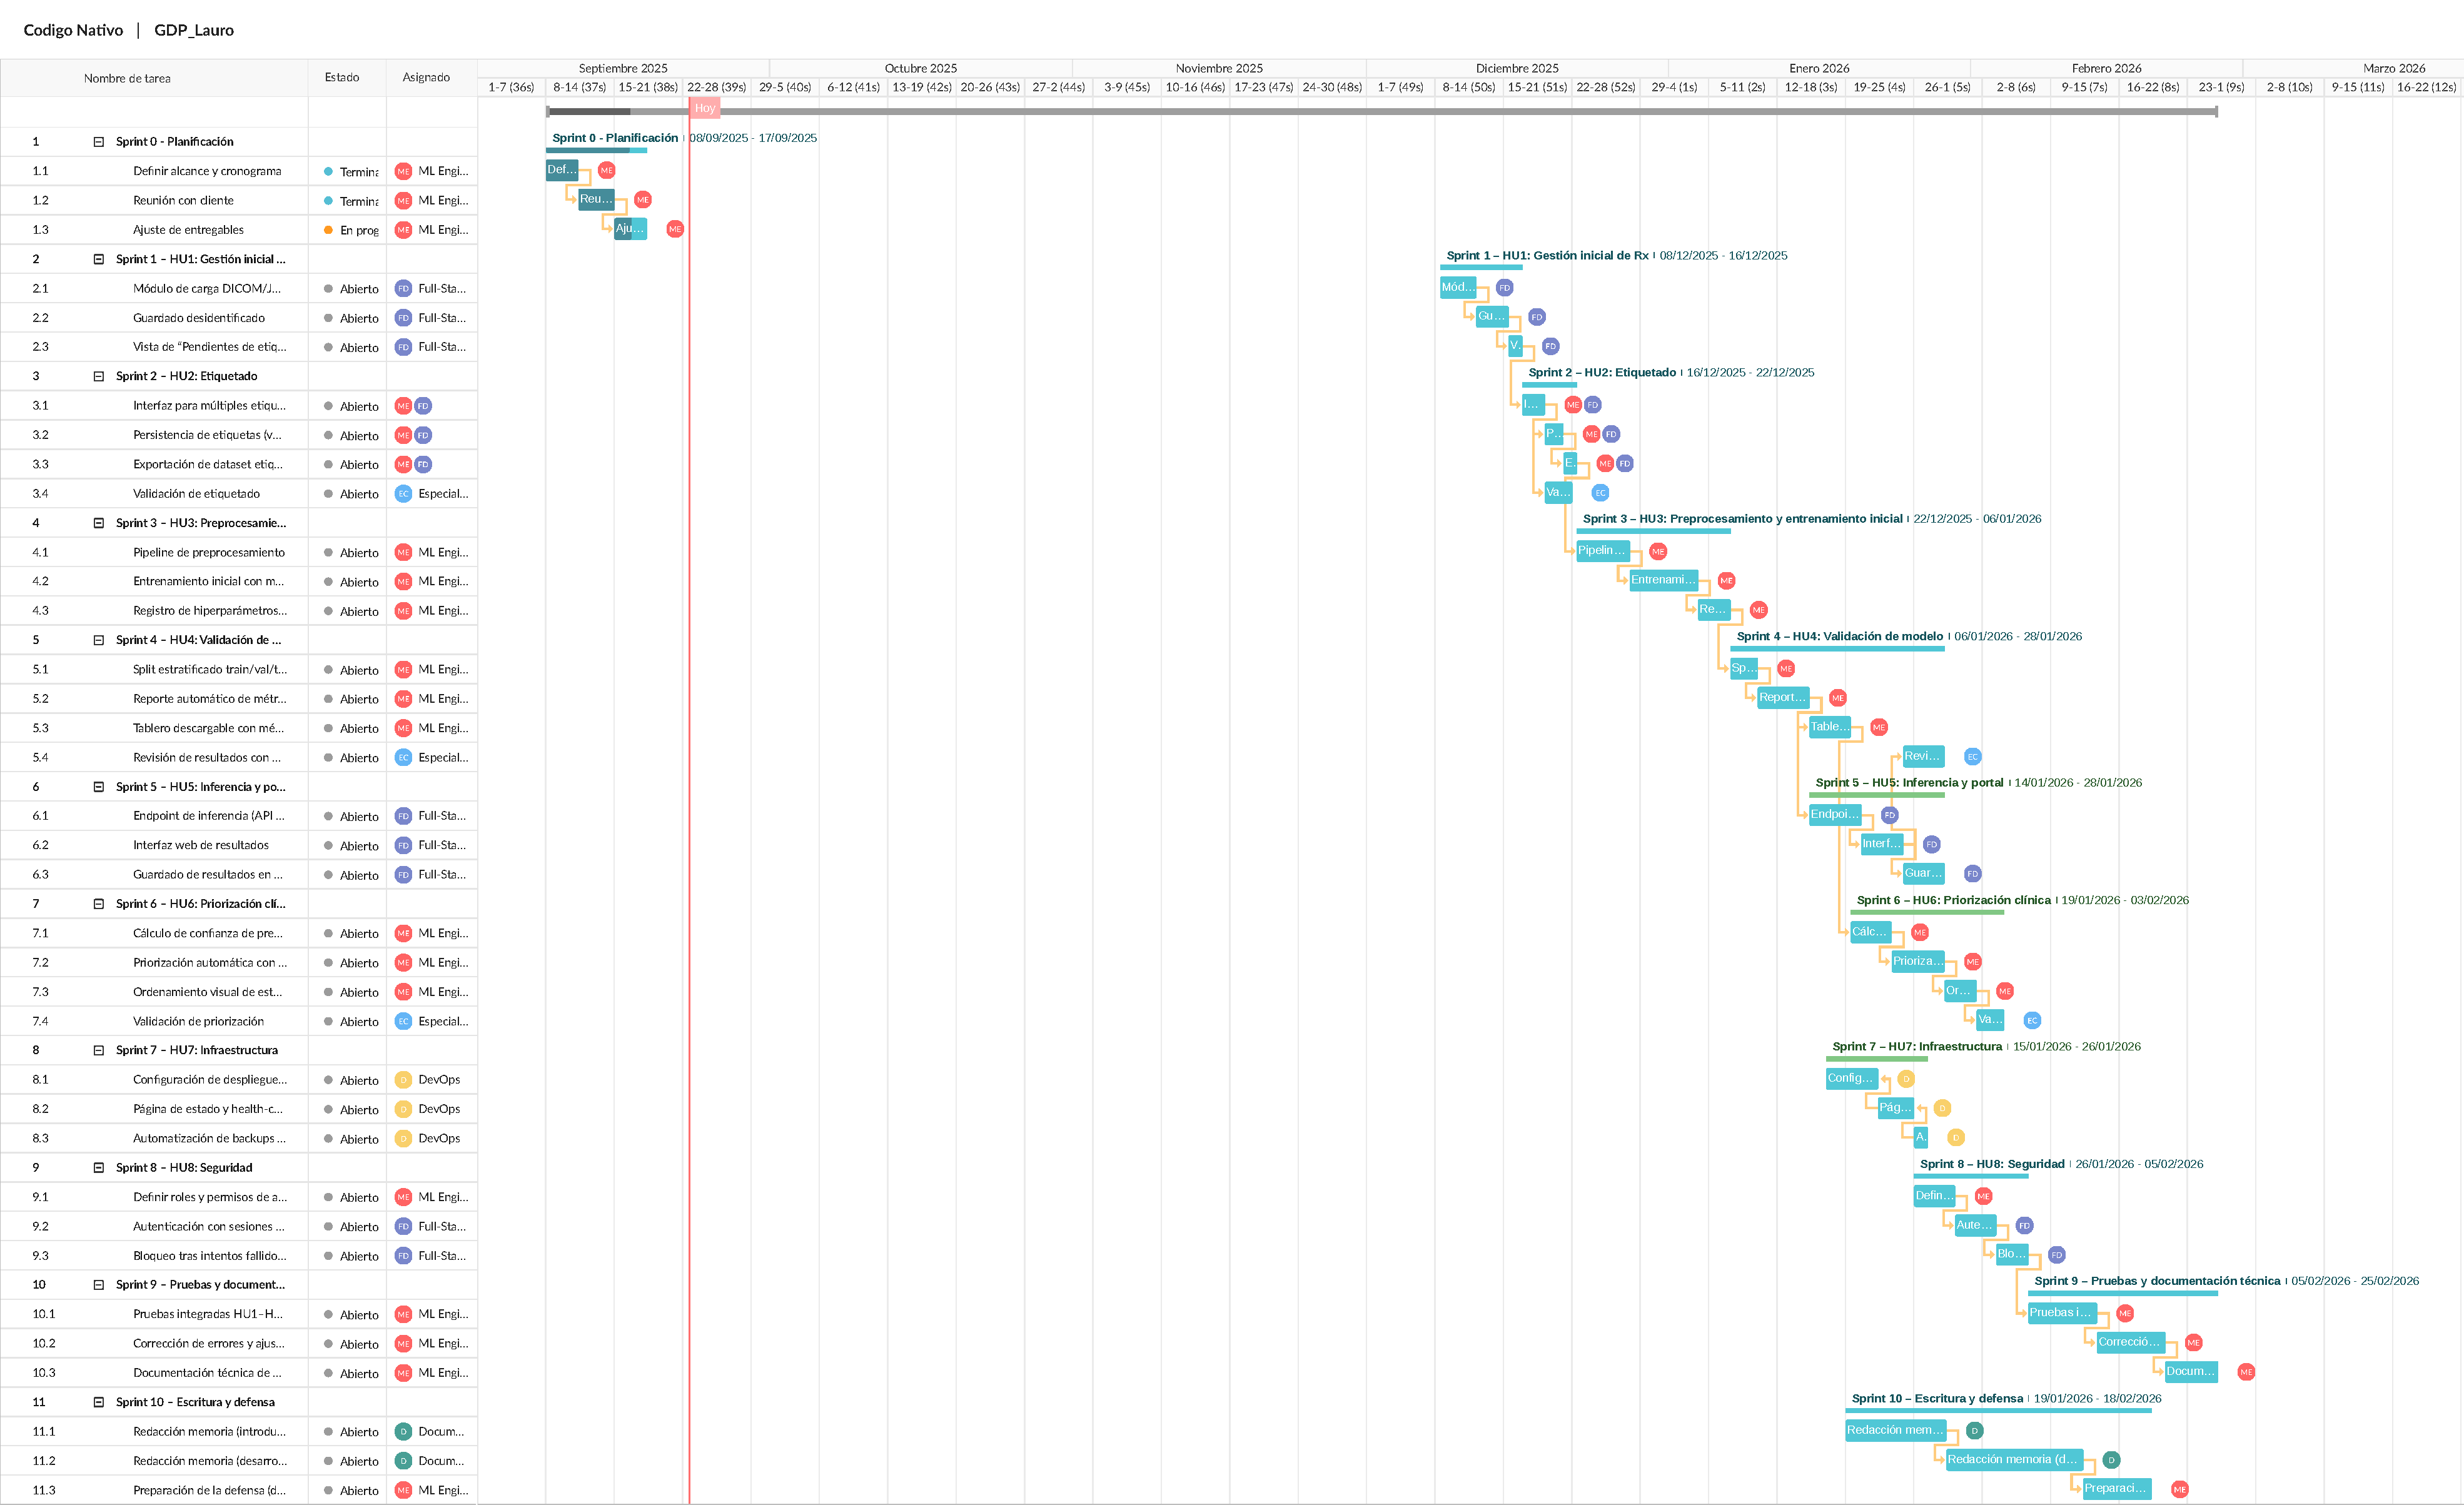
\includegraphics[angle=90,width=0.95\linewidth]{gantt.pdf}
    \label{fig:gantt}
\end{figure}





\section{12. Normativa y cumplimiento de datos (gobernanza)}


Los datos empleados en este proyecto consisten en radiografías de tórax de pacientes atendidos en el Hospital de Clínicas. Al tratarse de \textbf{imágenes médicas vinculadas a información de salud}, están sujetos a normativas nacionales e internacionales sobre privacidad y protección de datos.  

\subsection*{Normativas aplicables}
\begin{itemize}
    \item \textbf{Ley 25.326 de Protección de Datos Personales (Argentina)}: regula el tratamiento de datos sensibles, entre ellos los vinculados a la salud. Establece la obligación de anonimizar la información y de contar con consentimiento informado o autorización institucional para su uso.
    \item \textbf{GDPR (Unión Europea)}: aunque no aplica directamente, se toma como referencia de buenas prácticas por su estándar internacional. Requiere principios de licitud, minimización y limitación de la finalidad.
    \item \textbf{HIPAA (EE.UU.)}: normativa relevante para proyectos que involucren intercambio internacional de datos médicos. Se contempla como marco de referencia.
\end{itemize}

\subsection*{Condiciones de uso de los datos}
\begin{itemize}
    \item El acceso a las radiografías se encuentra regulado y autorizado institucionalmente.
    \item Las imágenes se emplean \textbf{únicamente con fines académicos} y de investigación, sin propósitos comerciales.
    \item Previo a su uso, los datos son \textbf{desidentificados} (eliminación de nombres, DNI, historia clínica u otros identificadores).
    \item No se comparten públicamente las imágenes originales: sólo se utiliza un subconjunto con autorización expresa del Hospital, y en los informes se publican métricas y resultados agregados.
\end{itemize}

\subsection*{Restricciones y consideraciones}
\begin{itemize}
    \item Cualquier publicación derivada del proyecto (artículos, memoria académica, presentaciones) incluirá únicamente datos anonimizados y resultados estadísticos.
    \item No se almacenan identificadores personales en las bases de datos del proyecto.
    \item Se asume que el Hospital de Clínicas garantiza el marco legal del consentimiento de los pacientes al momento de generar las imágenes.
\end{itemize}

\subsection*{Gobernanza y viabilidad}
\begin{itemize}
    \item Se adopta un esquema de \textbf{gobernanza de datos} donde el Hospital de Clínicas es el custodio de la información y el equipo académico es usuario autorizado.
    \item Se aplican medidas de seguridad técnicas (cifrado en reposo y en tránsito, control de accesos) y organizativas (roles definidos, auditoría).
    \item Desde el punto de vista legal y ético, el proyecto resulta viable siempre que se mantenga la desidentificación estricta, la trazabilidad del uso de datos y la confidencialidad.
\end{itemize}



\section{13. Gestión de riesgos}
\label{sec:riesgos}

\begin{consigna}{red}
a) Identificación de los riesgos (al menos cinco) y estimación de sus consecuencias:
 
Riesgo 1: detallar el riesgo (riesgo es algo que si ocurre altera los planes previstos de forma negativa)
\begin{itemize}
	\item Severidad (S): mientras más severo, más alto es el número (usar números del 1 al 10).\\
	Justificar el motivo por el cual se asigna determinado número de severidad (S).
	\item Probabilidad de ocurrencia (O): mientras más probable, más alto es el número (usar del 1 al 10).\\
	Justificar el motivo por el cual se asigna determinado número de (O). 
\end{itemize}   

Riesgo 2:
\begin{itemize}
	\item Severidad (S): X.\\
	Justificación...
	\item Ocurrencia (O): Y.\\
	Justificación...
\end{itemize}

Riesgo 3:
\begin{itemize}
	\item Severidad (S):  X.\\
	Justificación...
	\item Ocurrencia (O): Y.\\
	Justificación...
\end{itemize}


b) Tabla de gestión de riesgos:      (El RPN se calcula como RPN=SxO)

\begin{table}[htpb]
\centering
\begin{tabularx}{\linewidth}{@{}|X|c|c|c|c|c|c|@{}}
\hline
\rowcolor[HTML]{C0C0C0} 
Riesgo & S & O & RPN & S* & O* & RPN* \\ \hline
       &   &   &     &    &    &      \\ \hline
       &   &   &     &    &    &      \\ \hline
       &   &   &     &    &    &      \\ \hline
       &   &   &     &    &    &      \\ \hline
       &   &   &     &    &    &      \\ \hline
\end{tabularx}%
\end{table}

Criterio adoptado: 

Se tomarán medidas de mitigación en los riesgos cuyos números de RPN sean mayores a...

Nota: los valores marcados con (*) en la tabla corresponden luego de haber aplicado la mitigación.

c) Plan de mitigación de los riesgos que originalmente excedían el RPN máximo establecido:
 
Riesgo 1: plan de mitigación (si por el RPN fuera necesario elaborar un plan de mitigación).
  Nueva asignación de S y O, con su respectiva justificación:
  \begin{itemize}
	\item Severidad (S*): mientras más severo, más alto es el número (usar números del 1 al 10).
          Justificar el motivo por el cual se asigna determinado número de severidad (S).
	\item Probabilidad de ocurrencia (O*): mientras más probable, más alto es el número (usar del 1 al 10).
          Justificar el motivo por el cual se asigna determinado número de (O).
	\end{itemize}

Riesgo 2: plan de mitigación (si por el RPN fuera necesario elaborar un plan de mitigación).
 
Riesgo 3: plan de mitigación (si por el RPN fuera necesario elaborar un plan de mitigación).

\end{consigna}

\section{14. Sprint Review}
\label{sec:sprint_review}

La revisión de sprint (\emph{Sprint Review}) es una práctica fundamental en metodologías ágiles. Consiste en revisar y evaluar lo que se ha completado al finalizar un sprint. En esta instancia, se presentan los avances y se verifica si las funcionalidades cumplen con los criterios de aceptación establecidos. También se identifican entregables parciales y se consideran ajustes si es necesario.

Aunque el proyecto aún se encuentre en etapa de planificación, esta sección permite proyectar cómo se evaluarán las funcionalidades más importantes del backlog. Esta mirada anticipada favorece la planificación enfocada en valor y permite reflexionar sobre posibles obstáculos.

\textbf{Objetivo:} anticipar cómo se evaluará el avance del proyecto a medida que se desarrollen las funcionalidades, utilizando como base al menos cuatro historias de usuario del \emph{Product Backlog}.


Seleccionar al menos 4 HU del Product Backlog. Para cada una, completar la siguiente tabla de revisión proyectada:

\textbf{Formato sugerido:}
\begin{table}[htpb]
\renewcommand{\arraystretch}{1.5}
\begin{tabular}{|>{\raggedright\arraybackslash}m{2.4cm}|
                >{\raggedright\arraybackslash}m{2.3cm}|
                >{\raggedright\arraybackslash}m{3cm}|
                >{\raggedright\arraybackslash}m{3cm}|
                >{\raggedright\arraybackslash}m{3cm}|}
\hline
\rowcolor[HTML]{CCCCCC}
\textbf{HU seleccionada} & \textbf{Tareas asociadas} & \textbf{Entregable esperado} & \textbf{¿Cómo sabrás que está cumplida?} & \textbf{Observaciones o riesgos} \\
\hline
                         & Tarea 1 &                             &                                           &                                     \\ \cline{2-2}
\multirow{-2}{=}{HU1}    & Tarea 2 & \multirow{-2}{=}{Módulo funcional} & \multirow{-2}{=}{Cumple criterios de aceptación definidos} & \multirow{-2}{=}{Falta validar con el tutor} \\
\hline
                         & Tarea 1 &                             &                                           &                                     \\ \cline{2-2}
\multirow{-2}{=}{HU3}    & Tarea 2 & \multirow{-2}{=}{Reporte generado} & \multirow{-2}{=}{Exportación disponible y clara} & \multirow{-2}{=}{Requiere datos reales} \\
\hline
                         & Tarea 1 &                             &                                           &                                     \\ \cline{2-2}
\multirow{-2}{=}{HU5}    & Tarea 2 & \multirow{-2}{=}{Panel de gestión} & \multirow{-2}{=}{Roles diferenciados operativos} & \multirow{-2}{=}{Riesgo en integración} \\
\hline
                         & Tarea 1 &                             &                                           &                                     \\ \cline{2-2}
\multirow{-2}{=}{HU7}    & Tarea 2 & \multirow{-2}{=}{Informe trimestral} & \multirow{-2}{=}{PDF con gráficos y evolución} & \multirow{-2}{=}{Puede faltar tiempo para ajustes} \\
\hline
\end{tabular}
\end{table}

\section{15. Sprint Retrospective}    
\label{sec:sprint_retro}

La retrospectiva de sprint es una práctica orientada a la mejora continua. Al finalizar un sprint, el equipo (o el Ing. Lauro, si trabaja de forma individual) reflexiona sobre lo que funcionó bien, lo que puede mejorarse y qué acciones concretas pueden implementarse para trabajar mejor en el futuro.

Durante la cursada se propuso el uso de la \textbf{Estrella de la Retrospectiva}, que organiza la reflexión en torno a cinco ejes:

\begin{itemize}
\item  ¿Qué hacer más?
\item  ¿Qué hacer menos?
\item  ¿Qué mantener?
\item  ¿Qué empezar a hacer?
\item  ¿Qué dejar de hacer?
\end{itemize}

Aun en una etapa temprana, esta herramienta permite que el Ing. Lauro planifique su forma de trabajar, identifique anticipadamente posibles dificultades y diseñe estrategias de organización personal.

\textbf{Objetivo:} reflexionar sobre las condiciones iniciales del proyecto, identificando fortalezas, posibles dificultades y estrategias de mejora, incluso antes del inicio del desarrollo.


Completar la siguiente tabla tomando como referencia los cinco ejes de la Estrella de la Retrospectiva (\emph{Starfish} o estrella de mar). Esta instancia te ayudará a definir buenas prácticas desde el inicio y prepararte para enfrentar el trabajo de forma organizada y flexible. Se deberá completar la tabla al menos para 3 sprints técnicos y 1 no técnico.

\textbf{Formato sugerido:}

\begin{table}[htpb]
\renewcommand{\arraystretch}{1.4}
\begin{tabular}{|>{\raggedright\arraybackslash}p{1.8cm}|
                >{\raggedright\arraybackslash}p{2.3cm}|
                >{\raggedright\arraybackslash}p{2.3cm}|
                >{\raggedright\arraybackslash}p{2.3cm}|
                >{\raggedright\arraybackslash}p{2.3cm}|
                >{\raggedright\arraybackslash}p{2.3cm}|}
\hline
\rowcolor[HTML]{CCCCCC} 
\textbf{Sprint tipo y N°} & \textbf{¿Qué hacer más?} & \textbf{¿Qué hacer menos?} & \textbf{¿Qué mantener?} & \textbf{¿Qué empezar a hacer?} & \textbf{¿Qué dejar de hacer?} \\
\hline
Sprint técnico - 1 & Validaciones continuas con el Ing. Lauro & Cambios sin versión registrada & Pruebas con datos simulados & Documentar cambios propuestos & Ajustes sin análisis de impacto \\
\hline
Sprint técnico - 2 & Verificar configuraciones en múltiples escenarios & Modificar parámetros sin guardar historial & Perfiles reutilizables & Usar logs para configuración & Repetir pruebas manuales innecesarias \\
\hline
Sprint técnico - 8 & Comparar correlaciones con casos previos & Cambiar parámetros sin justificar & Revisión cruzada de métricas & Anotar configuraciones usadas & Trabajar sin respaldo de datos \\
\hline
Sprint no técnico - 12 (por ej.: ``Defensa'') & Ensayos orales con feedback & Cambiar contenidos en la memoria & Material visual claro & Dividir la presentación por bloques & Agregar gráficos difíciles de explicar \\
\hline
\end{tabular}
\end{table}




\end{document}